\documentclass[10pt,a4paper,titlepage]{report}
\usepackage[utf8]{inputenc}
\usepackage[portuguese]{babel}
\usepackage[T1]{fontenc}
\usepackage{amsmath}
\usepackage{amsfonts}
\usepackage{amssymb}
\usepackage{graphicx}
\usepackage[left=1cm, right=1cm]{geometry}
\usepackage[nottoc]{tocbibind}
\usepackage{multicol}
\usepackage{titlepic}
\begin{document}

\pagenumbering{Roman}
\author{António Maria Faria Nobre dos Santos Fróis\\Turma: TP11-51050, Nr: 51050\\e-mail: antoniofarois@hotmail.com}
\title{Trabalho de Produção de Documentos Técnicos}
\titlepic{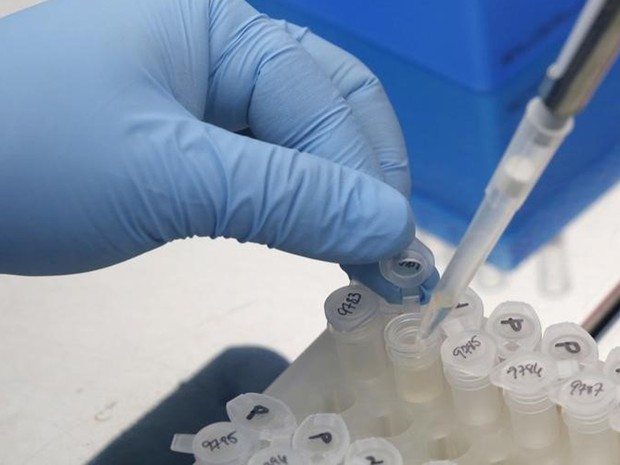
\includegraphics[scale=0.5]{Icapa.png}}
\thispagestyle{empty}
\maketitle
\tableofcontents
\chapter{Introdução}
	Hoje em dia todos somos vacinados sem sabermos o que são realmente as vacinas ou como estas verdadeiramente atuam, assim sendo o que são realmente as vacinas, para que servem e quais as suas desvantagens e vantagens? Uma vacina, cientificamente falando, é a introdução de uma substância(vírus ou bactéria), estando esta já desativada ou quase morta, no corpo de um ser vivo. Esta substância é introduzida no corpo do ser vivo com o objetivo de estimular o sistema imunológico a produzir anticorpos conta a mesma, uma vez vacinado, caso a bactéria ou vírus volte a entrar em contacto com o corpo do ser vivo, o seu sistema ja é capaz de reconhecer e eliminar imediatamente a substância. As vacinas dividem-se em três tipos: as de DNA onde se insere no ser vivo apenas partes do genoma do vírus ou bactéria, as vivas, em que o vírus é atenuado, ou seja, a substância injetada no sujeito está vivo mas não podendo causar doença e as mortas onde a bactéria está morta. Apesar de parecer que as vacinas são apenas vantajosas isto não é verdade, estas possuem também as suas desvantagens, vamos então comparar as vantagens e desvantagens das mesmas nas duas colunas abaixo, respetivamente:
\vspace{1cm}

 \begin{minipage}[t]{7cm}
 	Quando o agente infeccioso que é inserido no corpo de um indivíduo está vivo, a imunidade que é adquirida ao agente é mais duradoura do que caso ele estivesse morto ou inativo, o que acontece pois o agente mimetiza uma infeção natural, isto é, o vírus ou bactéria imita uma infeção natural, o que para além da vantagem referida acima faz com que a imunidade celular também melhore, este tipo de vacinas permite também uma vacinação em grande escala, ou seja, pode ser usada em muitas doenças e gripes. 
 \end{minipage}
 \hspace{2cm}
 \begin{minipage}[t]{7cm}
 	Quando no ato de vacinação a substância introduzida no ser vivo está adormecida, ou seja, não está completamente morta, e ganha formas infecciosas graves, a pessoa vacinada corre o risco de ser infectada e ter efeitos colaterais graves; nem todas as vacinas podem ser administradas em toda a gente, por exemplo, pessoas com doenças neurológicas; se o indivíduo estiver doente com febre (temperaturas superiores a 38,5ºC),  a vacinação não deverá ser feita nessa altura tendo que ser adiada; após administração da vacina podem-se verificar efeitos secundários como febre, dor, síncopes, estes ocorrendo dentro das primeiras 24 horas e em certos casos podem causar dano cerebral significante, o que, felizmente, acontece apenas raramente; há também determinados tipos de vacinas cujos efeitos não são muito duradouros, sendo assim necessário mais administrações num menor espaço de tempo.
  \end{minipage}
\chapter{Caso de estudo}
	Os próximos gráficos e tabelas são relativos ao estudo da avaliação do número de trabalhadores, onde se pretende avaliar se estes são suficientes, estão a mais ou a menos, sendo esta feita através dos valores da  percentagem da ocupação da mão-de-obra. No estudo apresentado, os valores de produtividade são de 151 encomendas por trabalhador e o número de trabalhadores é 405 (gráfico \ref{G1} e tabela \ref{T1}) e 435 trabalhadores (gráfico \ref{G2} e tabela \ref{T2}).
\begin{center}
\begin{table}
	\begin{tabular}{ | c | c | c | c | c | c | c | c | }
		\hline
		\multicolumn{1}{|c|}{Dia} & \multicolumn{1}{c|}{\begin{tabular}[c]{@{}c@{}}Nº\\ Aleatório\end{tabular}} & \multicolumn{1}{c|}{\begin{tabular}[c]{@{}c@{}}Nº de\\  Encomendas\\ Recebidas\end{tabular}} & \multicolumn{1}{c|}{\begin{tabular}[c]{@{}c@{}}Nºde\\  Encomendas\\ a Produzir\end{tabular}} & \multicolumn{1}{c|}{\begin{tabular}[c]{@{}c@{}}Capacidade \\ de \\ Produção Diária\end{tabular}} & \multicolumn{1}{c|}{\begin{tabular}[c]{@{}c@{}}Nº de \\ Encomendas\\ Produzidas\end{tabular}} & \multicolumn{1}{c|}{\begin{tabular}[c]{@{}c@{}}Nº de \\ Encomendas\\ em Atraso\end{tabular}} & \multicolumn{1}{c|}{\begin{tabular}[c]{@{}c@{}}Percentagem da \\ Ocupação\\ da mão-de-obra\end{tabular}} \\ \hline
		1 & 0.49 & 60000 & 60000 & 61555 & 61555 & 0 & 1 \\ \hline
		2 & 0.94 & 70000 & 70000 & 61555 & 61555 & 8445 & 1 \\ \hline
		3 & 0.69 & 65000 & 73445 & 61555 & 61555 & 11890 & 1 \\ \hline
		4 & 0.7 & 65000 & 76890 & 61555 & 61555 & 15335 & 1 \\ \hline
		5 & 0.47 & 60000 & 75335 & 61555 & 61555 & 13780 & 1 \\ \hline
		6 & 0.76 & 65000 & 78780 & 61555 & 61555 & 17225 & 1 \\ \hline
		7 & 0.86 & 65000 & 82225 & 61555 & 61555 & 20670 & 1 \\ \hline
		8 & 0.4 & 60000 & 80670 & 61555 & 61555 & 19115 & 1 \\ \hline
		9 & 0.63 & 65000 & 84115 & 61555 & 61555 & 22560 & 1 \\ \hline
		10 & 0.19 & 55000 & 77560 & 61555 & 61555 & 16005 & 1 \\ \hline
		11 & 0.5 & 60000 & 76005 & 61555 & 61555 & 14450 & 1 \\ \hline
		12 & 0.54 & 60000 & 74450 & 61555 & 61555 & 12895 & 1 \\ \hline
		13 & 0.37 & 60000 & 72895 & 61555 & 61555 & 11340 & 1 \\ \hline
		14 & 0.54 & 60000 & 71340 & 61555 & 61555 & 9785 & 1 \\ \hline
		15 & 0.76 & 65000 & 74785 & 61555 & 61555 & 13230 & 1 \\ \hline
		16 & 0.08 & 50000 & 63230 & 61555 & 61555 & 1675 & 1 \\ \hline
		17 & 0.41 & 60000 & 61675 & 61555 & 61555 & 120 & 1 \\ \hline
		18 & 0.36 & 60000 & 60120 & 61555 & 60120 & 0 & 0.97668751523028186 \\ \hline
		19 & 0.13 & 50000 & 50000 & 61555 & 50000 & 0 & 0.81228169929331495 \\ \hline
		20 & 0.8 & 65000 & 65000 & 61555 & 61555 & 3445 & 1 \\ \hline
		21 & 0.25 & 55000 & 58445 & 61555 & 58445 & 0 & 0.94947607830395586 \\ \hline
		22 & 0.78 & 65000 & 65000 & 61555 & 61555 & 3445 & 1 \\ \hline
		23 & 0.76 & 65000 & 68445 & 61555 & 61555 & 6890 & 1 \\ \hline
		24 & 0.77 & 65000 & 71890 & 61555 & 61555 & 10335 & 1 \\ \hline
		25 & 0.76 & 65000 & 75335 & 61555 & 61555 & 13780 & 1 \\ \hline
		26 & 0.59 & 60000 & 73780 & 61555 & 61555 & 12225 & 1 \\ \hline
		27 & 0.4 & 60000 & 72225 & 61555 & 61555 & 10670 & 1 \\ \hline
		28 & 0.05 & 50000 & 60670 & 61555 & 60670 & 0 & 0.98562261392250827 \\ \hline
		29 & 0.02 & 50000 & 50000 & 61555 & 50000 & 0 & 0.81228169929331495 \\ \hline
		30 & 0.63 & 65000 & 65000 & 61555 & 61555 & 3445 & 1 \\ \hline
	\end{tabular}
\caption{Tabela do caso onde se contratam 405 trabalhadores}
\label{T1}
\end{table}

\begin{figure}[h]
\begin{center}
	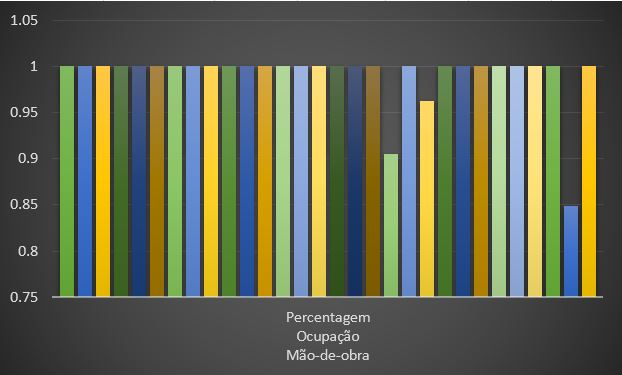
\includegraphics[scale=1]{G1.png}
	\caption{Gráfico da Percentagem da Ocupação da mão-de-obra com 405 trabalhadores}
	\label{G1}
\end{center}
\end{figure}
\end{center}
\begin{center}
\begin{figure}[h]	
\begin{center}
	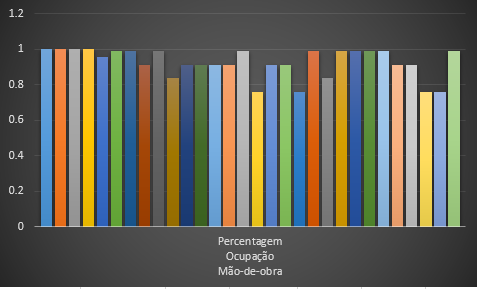
\includegraphics[scale=1]{GOtimizado.PNG}
	\caption{Gráfico Otimizado da Percentagem da Ocupação da mão-de-obra}
	\label{G2}
\end{center}
\end{figure}
\begin{table}
\begin{tabular}{ | c | c | c | c | c | c | c | c | c | c | c | c | c | }
\hline
	\multicolumn{1}{|c|}{Dia} & \multicolumn{1}{c|}{\begin{tabular}[c]{@{}c@{}}Nº\\ Aleatório\end{tabular}} & \multicolumn{1}{c|}{\begin{tabular}[c]{@{}c@{}}Nº de\\  Encomendas\\ Recebidas\end{tabular}} & \multicolumn{1}{c|}{\begin{tabular}[c]{@{}c@{}}Nºde\\  Encomendas\\ a Produzir\end{tabular}} & \multicolumn{1}{c|}{\begin{tabular}[c]{@{}c@{}}Capacidade \\ de \\ Produção Diária\end{tabular}} & \multicolumn{1}{c|}{\begin{tabular}[c]{@{}c@{}}Nº de \\ Encomendas\\ Produzidas\end{tabular}} & \multicolumn{1}{c|}{\begin{tabular}[c]{@{}c@{}}Nº de \\ Encomendas\\ em Atraso\end{tabular}} & \multicolumn{1}{c|}{\begin{tabular}[c]{@{}c@{}}Percentagem da \\ Ocupação\\ da mão-de-obra\end{tabular}} \\ \hline
	1 & 0.49 & 60000 & 60000 & 65685 & 65685 & 0 & 1 \\ \hline
	2 & 0.94 & 70000 & 70000 & 65685 & 65685 & 4315 & 1 \\ \hline
	3 & 0.69 & 65000 & 69315 & 65685 & 65685 & 3630 & 1  \\ \hline
	4 & 0.7 & 65000 & 68630 & 65685 & 65685 & 2945 & 1  \\ \hline
	5 & 0.47 & 60000 & 62945 & 65685 & 62945 & 0 & 0.95828575778336 \\ \hline
	6 & 0.76 & 65000 & 65000 & 65685 & 65000 & 0 & 0.98957143944584003  \\ \hline
	7 & 0.86 & 65000 & 65000 & 65685 & 65000 & 0 & 0.98957143944584003  \\ \hline
	8 & 0.4 & 60000 & 60000 & 65685 & 60000 & 0 & 0.91345055948846765  \\ \hline
	9 & 0.63 & 65000 & 65000 & 65685 & 65000 & 0 & 0.98957143944584003  \\ \hline
	10 & 0.19 & 55000 & 55000 & 65685 & 55000 & 0 & 0.83732967953109538 \\ \hline
	11 & 0.5 & 60000 & 60000 & 65685 & 60000 & 0 & 0.91345055948846765  \\ \hline
	12 & 0.54 & 60000 & 60000 & 65685 & 60000 & 0 & 0.91345055948846765  \\ \hline
	13 & 0.37 & 60000 & 60000 & 65685 & 60000 & 0 & 0.91345055948846765  \\ \hline
	14 & 0.54 & 60000 & 60000 & 65685 & 60000 & 0 & 0.91345055948846765  \\ \hline
	15 & 0.76 & 65000 & 65000 & 65685 & 65000 & 0 & 0.98957143944584003  \\ \hline
	16 & 0.08 & 50000 & 50000 & 65685 & 50000 & 0 & 0.76120879957372312  \\ \hline
	17 & 0.41 & 60000 & 60000 & 65685 & 60000 & 0 & 0.91345055948846765  \\ \hline
	18 & 0.36 & 60000 & 60000 & 65685 & 60000 & 0 & 0.91345055948846765  \\ \hline
	19 & 0.13 & 50000 & 50000 & 65685 & 50000 & 0 & 0.76120879957372312  \\ \hline
	20 & 0.8 & 65000 & 65000 & 65685 & 65000 & 0 & 0.98957143944584003  \\ \hline
	21 & 0.25 & 55000 & 55000 & 65685 & 55000 & 0 & 0.83732967953109538  \\ \hline
	22 & 0.78 & 65000 & 65000 & 65685 & 65000 & 0 & 0.98957143944584003  \\ \hline
	23 & 0.76 & 65000 & 65000 & 65685 & 65000 & 0 & 0.98957143944584003  \\ \hline
	24 & 0.77 & 65000 & 65000 & 65685 & 65000 & 0 & 0.98957143944584003  \\ \hline
	25 & 0.76 & 65000 & 65000 & 65685 & 65000 & 0 & 0.98957143944584003  \\ \hline
	26 & 0.59 & 60000 & 60000 & 65685 & 60000 & 0 & 0.91345055948846765  \\ \hline
	27 & 0.4 & 60000 & 60000 & 65685 & 60000 & 0 & 0.91345055948846765  \\ \hline
	28 & 0.05 & 50000 & 50000 & 65685 & 50000 & 0 & 0.76120879957372312  \\ \hline
	29 & 0.02 & 50000 & 50000 & 65685 & 50000 & 0 & 0.76120879957372312 \\ \hline
	30 & 0.63 & 65000 & 65000 & 65685 & 65000 & 0 & 0.98957143944584003 \\ \hline
\end{tabular}
\caption{Tabela otimizada do caso onde se contratam 435 trabalhadores}
\label{T2}
\end{table}
\end{center}
\chapter{Conclusão}
	Concluindo o número de trabalhadores que é usado na tabela \ref{T2}, ou seja, o que eu escolhi, dado as condições é o mais adequado pois é onde se verifica uma média da percentagem da ocupação da mão-de-obra superior a 90\% e o número de encomendas em atraso é mínimo. Caso aumentássemos o número de trabalhadores, as encomendas em atraso diminuiam e o mesmo acontecia à percentagem de ocupação da mão-de-obra sendo esta inferior a 90\%; caso diminuíssemos o número de trabalhadores o contrário aconteceria, isto é, a percentagem de ocupação da mão-de-obra aumentava mas haveria mais encomendas em atraso. Comparando os gráficos \ref{G1} e \ref{G2} é possível verificar que quando o número de trabalhadores aumenta a percentagem de ocupação da mão-de-obra diminui. Analisando agora as tabelas \ref{T1} e \ref{T2}, comparando as colunas do Nº de encomendas em atraso, verifica-se que este diminui com o acréscimo de trabalhadores. Estas duas comparações verificam o que foi acima escrito logo o número de trabalhadores escolhido nunca será o ideal mas o que é apresentado na tabela \ref{T2} e no gráfico \ref{G2} é o que melhor se adequa ao caso de estudo apresentado.

\bibliography{Trabalho}
\bibliographystyle{plain}
\nocite{Imagem_Capa}
\nocite{Significado_Vacina}
\nocite{Vacina_para_que_serve}
\nocite{Vantagens_Desvantagens1}
\nocite{Vantagens_Desvantagens2}
\nocite{Vantagens_Desvantagens3}
\end{document}